\documentclass[12pt]{article}
%%%%%%%%%%%%%%%%
% Packages
%%%%%%%%%%%%%%%%

\usepackage[top=1cm,bottom=1cm,left=1.5cm,right= 1.5cm]{geometry}
\usepackage[parfill]{parskip}
\usepackage{graphicx, fontspec, xcolor, multicol, enumitem, setspace}
\DeclareGraphicsRule{.tif}{png}{.png}{`convert #1 `dirname #1`/`basename #1 .tif`.png}

%%%%%%%%%%%%%%%%
% Sakai link - update each semester
%%%%%%%%%%%%%%%%

\newcommand{\Sakai}[1]
{\href{https://sakai.duke.edu/portal/site/ef372254-413e-42f6-b414-f8bc91a58fa0/page/98390abf-b461-44cb-a062-aa6864748ab3}{Sakai}}


%%%%%%%%%%%%%%%%
% No page number
%%%%%%%%%%%%%%%%

\pagestyle{empty}

%%%%%%%%%%%%%%%%
% User defined colors
%%%%%%%%%%%%%%%%

% Pantone 2015 Spring colors
% http://iwork3.us/2014/09/16/pantone-2015-spring-fashion-report/
% update each semester or year

\xdefinecolor{custom_blue}{rgb}{0, 0.70, 0.79} % scuba blue
\xdefinecolor{custom_darkBlue}{rgb}{0.11, 0.31, 0.54} % classic blue
\xdefinecolor{custom_orange}{rgb}{0.97, 0.57, 0.34} % tangerine
\xdefinecolor{custom_green}{rgb}{0.49, 0.81, 0.71} % lucite green
\xdefinecolor{custom_red}{rgb}{0.58, 0.32, 0.32} % marsala

\xdefinecolor{custom_lightGray}{rgb}{0.78, 0.80, 0.80} % glacier gray
\xdefinecolor{custom_darkGray}{rgb}{0.54, 0.52, 0.53} % titanium

%%%%%%%%%%%%%%%%
% Color text commands
%%%%%%%%%%%%%%%%

%orange
\newcommand{\orange}[1]{\textit{\textcolor{custom_orange}{#1}}}

% yellow
\newcommand{\yellow}[1]{\textit{\textcolor{yellow}{#1}}}

% blue
\newcommand{\blue}[1]{\textit{\textcolor{blue}{#1}}}

% green
\newcommand{\green}[1]{\textit{\textcolor{custom_green}{#1}}}

% red
\newcommand{\red}[1]{\textit{\textcolor{custom_red}{#1}}}

%%%%%%%%%%%%%%%%
% Coloring titles, links, etc.
%%%%%%%%%%%%%%%%

\usepackage{titlesec}
\titleformat{\section}
{\color{custom_blue}\normalfont\Large\bfseries}
{\color{custom_blue}\thesection}{1em}{}
\titleformat{\subsection}
{\color{custom_blue}\normalfont}
{\color{custom_blue}\thesubsection}{1em}{}

\newcommand{\ttl}[1]{ \textsc{{\LARGE \textbf{{\color{custom_blue} #1} } }}}

\newcommand{\tl}[1]{ \textsc{{\large \textbf{{\color{custom_blue} #1} } }}}

\usepackage[colorlinks=false,pdfborder={0 0 0},urlcolor= custom_orange,colorlinks=true,linkcolor= custom_orange, citecolor= custom_orange,backref=true]{hyperref}

%%%%%%%%%%%%%%%%
% Instructions box
%%%%%%%%%%%%%%%%

\newcommand{\inst}[1]{
\colorbox{custom_blue!20!white!50}{\parbox{\textwidth}{
	\vskip10pt
	\leftskip10pt \rightskip10pt
	#1
	\vskip10pt
}}
\vskip10pt
}


%%%%%%%%%%%
% App Ex number    %
%%%%%%%%%%%

% DON'T FORGET TO UPDATE

\newcommand{\appno}[1]
{1.2}

%%%%%%%%%%%%%%
% Turn on/off solutions       %
%%%%%%%%%%%%%%

% Off
\newcommand{\soln}[1]{
\vskip5pt
}

%% On
%\newcommand{\soln}[1]{
%\textit{\textcolor{custom_darkGray}{#1}}
%}

%%%%%%%%%%%%%%%%
% Document
%%%%%%%%%%%%%%%%

\begin{document}
\fontspec[Ligatures=TeX]{Helvetica Neue Light}

Dr. \c{C}etinkaya-Rundel \hfill Data Analysis and Statistical Inference \\

\ttl{Application exercise \appno{}: \\
Distributions of numerical variables}

\inst{Submit your responses on \Sakai{}, under the appropriate assignment. Only one submission per team is required. One team will be randomly selected and their responses will be discussed.}

\tl{Shapes of distributions}

\begin{enumerate}

\item Below are two histograms. One corresponds to the age at which a sample of people applied for marriage licenses; the other corresponds to the last digit of a sample of social security numbers. Which graph is which, and why?

\begin{multicols}{2}

\begin{enumerate}

\item $\:$ \\
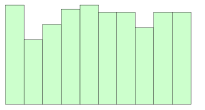
\includegraphics[height=1.1in]{figures/last_digit_SSN}

\item $\:$ \\
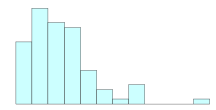
\includegraphics[height=1.1in]{figures/age_mar_lic}

\end{enumerate}

\end{multicols}

%

\item Match the following variables with the histograms and bar graphs given below. These data represent Sta 101 students at Duke. [\textit{Hint: Think about how each variable should behave.}]

\begin{multicols}{2}
\begin{enumerate}
\item the height of students
\item gender breakdown of students
\item the time it took students to get to their first class of the day
\item the number of hours of sleep students received last night
\item whether or not students live off campus
\item the number of piercings students have
\end{enumerate}
\end{multicols}


\begin{multicols}{3}

\begin{enumerate}

\item[(1)] $\:$ \\
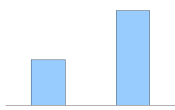
\includegraphics[height=1.1in]{figures/gender}

\item[(2)] $\:$ \\
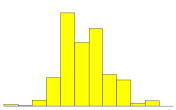
\includegraphics[height=1.1in]{figures/height}

\item[(3)] $\:$ \\
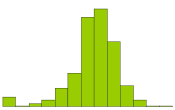
\includegraphics[height=1.1in]{figures/sleep}

\item[(4)] $\:$ \\
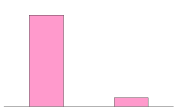
\includegraphics[height=1.1in]{figures/off_campus}

\item[(5)] $\:$ \\
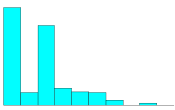
\includegraphics[height=1.1in]{figures/piercings}

\item[(6)] $\:$ \\
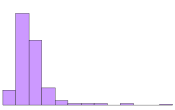
\includegraphics[height=1.1in]{figures/time_to_class}

\end{enumerate}

%

\end{multicols}

\item Come up with a concise way (1-2 sentences) to teach someone how to determine the expected distribution of any variable.

\end{enumerate}

%

\pagebreak

\tl{Variability}

\begin{enumerate}[resume]

\item[4.] Order histograms A, B, and C from least to most variable. Explain your reasoning.

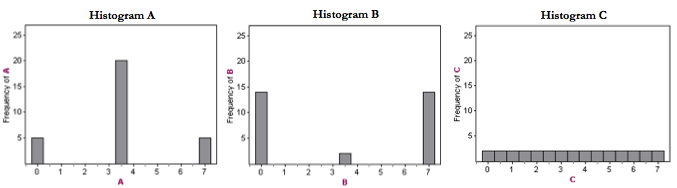
\includegraphics[width=0.9\textwidth]{figures/histogramsVarOrderABC}

$\:$ \\
$\:$ \\
$\:$ \\

\item[5.] Between histograms D and E, which exhibits more variability? Explain your reasoning.

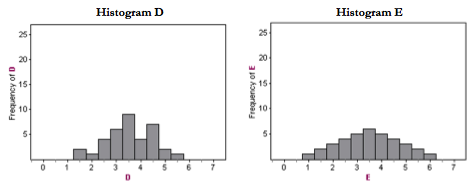
\includegraphics[width=0.9\textwidth]{figures/histogramsVarOrderDE}

\end{enumerate}


\end{document}